%%%%%%%%%%%%%%%%%%%%%%%%%%%%%%%%%%%%%%%%%%%%%%%%%%%%%%%%%%%%%%%%%%%%%%%%%%%%%%%
%
% Tool / Projet presentation template, by Quentin Bouvet (qbouvet@outlook.com)
%
% Based on "conference paper template, Food and Resource Economics Department -
% UNIVERSITY OF FLORIDA" By Ariel Soto-Caro (asotocaro@ufl.edu, arielsotocaro@
% gmail.com). Retrieved from overleaf in 2020.
%
%%%%%%%%%%%%%%%%%%%%%%%%%%%%%%%%%%%%%%%%%%%%%%%%%%%%%%%%%%%%%%%%%%%%%%%%%%%%%%%         

\documentclass[11pt]{article}
\usepackage{main}
\usepackage{lipsum}                     % Dummy text
\usepackage{listings}                   % Code formatting
\lstset{
   language=java,
   extendedchars=true,
   basicstyle=\footnotesize\ttfamily,
   showstringspaces=false,
   showspaces=false,
   numbers=left,
   numberstyle=\footnotesize,
   numbersep=9pt,
   tabsize=2,
   breaklines=true,
   showtabs=false,
   frame=single,
   extendedchars=false,
   inputencoding=utf8,
   captionpos=b
}
\usepackage{libertine}                  % Fonts (exp. for code formatting)
\usepackage[scaled=0.83]{beramono}
\usepackage{amssymb}                    % AMS math-packages
\usepackage{amsmath,amsthm}

\onehalfspacing % Line spacing {\doublespacing, singlespacing, \onehalfspacing}
\setlength{\droptitle}{-5em} %% Don't touch



%
%   Titles, Abstract and Table of Content
%

\title{
    GoFan: A maybe innovative, possibly \\
    useful way to control your computer fans
}

\author{\\% Name author
    \href{mailto:qbouvet@outlook.com}{\texttt{qbouvet@outlook.com}} %% Email author 1 
%\and Second Author\\% Name author
%    \href{mailto:secondauthor@ufl.edu}{\texttt{secondauthor@ufl.edu}} %% Email author 2
}
    
\date{\today}

\begin{document}

\setstretch{.8}
\maketitle

\begin{abstract}

When running a computer, variable fan speed allows silent operation under low load conditions by reducing the fan speed, and increases cooling capabilities under load by increasing the fan speed. Fan control is therefore a key issue for perfectionists who aim to design quiet computers. In this document, we present a new approach to fan control, which aims to lower acoustic disturbance to computer users. \\

Fan control is usually implemented using a fan curve, which temperatures to fan speed. Temperature is sampled at regular intervals, looked up to obtain a fan speed, which is then applied. This is run in a periodic loop. 
The issue with this approach is that due to the sample period usually being large (tyically 500-2000ms), it leads to big changes in fan speed, which are usually applied in 1 step. This generates brutal changes in noise levels, which are disturbing the computer users who want a silent system, while slower noise level change speed would be less noticeable and less disturbing to humans. \\

Our approach addresses this shortcomming by reducing the fan speed change rate, without compromissing on cooling reactivity. This is achieved with the following two techniques:
\begin{enumerate}
    \item We apply changes in fan speed in small steps over time, as opposed to one big periodic step, avoiding the brutal changes in noise levels perceived by the user,
    \item We predict the near-future temperatures of the system, allowing us to apply changes sooner, which gives us more time to apply the changes, reducing further the change rate in fan speed
\end{enumerate}
We also use hysteresis, a technique commonly used in other implementation to avoid some changes in fan speed when slowing down the fan.



% END CONTENT ABS------------------------------------------
%\noindent
%\textit{\textbf{Keywords: }%
%key1; key2; key3; key4.} \\ %% <-- Keywords HERE!
%\noindent
%\textit{\textbf{JEL Classification: }%
%Q12; C22; D81.} %% <-- JEL code HERE!
\end{abstract}


\tableofcontents

\newpage


%
%   Body 
%

%%\section{Overview}

\lipsum[2-1] % Dummy text. Erase before write
\citet{Hardaker2004} % Example of citation. Erase before use

\begin{table}[H]
    \centering
    \caption{Example table of descriptive statistics of the main variables.}
    \label{tab:1}
    \scalebox{.8}{
      \begin{tabular}{rlrrrrrr}
      \hline
      \multicolumn{1}{c}{\textbf{Variables}} & \multicolumn{1}{c}{\textbf{Categories}} & \multicolumn{1}{c}{\textbf{Unit}} & \multicolumn{1}{c}{\textbf{Rep}} & \multicolumn{1}{c}{\textbf{Mean}} & \multicolumn{1}{c}{\textbf{St. Dev.}} & \multicolumn{1}{c}{\textbf{Min}} & \multicolumn{1}{c}{\textbf{Max}} \\ \hline \hline
  
      \multicolumn{1}{l}{Variable 1} & Category A & \multicolumn{1}{c}{\$} & \multicolumn{1}{c}{8} & 0     & 0     & 0     & 0 \\
            & Category B & \multicolumn{1}{c}{lb} & \multicolumn{1}{c}{8} & 22,411.20 & 6,325.90 & 13,819 & 31,201 \\
            & Category C & \multicolumn{1}{c}{\$} & \multicolumn{1}{c}{8} & 5,869.60 & 4,609.90 & -464.1 & 12,744.10 \\
      \multicolumn{1}{l}{Variable 2} & Category A & \multicolumn{1}{c}{\$} & \multicolumn{1}{c}{8} & 1,777.40 & 144.5 & 1,642.30 & 1,912.60 \\
            & Category B & \multicolumn{1}{c}{lb} & \multicolumn{1}{c}{8} & 21,444.80 & 5,146.90 & 15,096 & 28,032 \\
            & Category C & \multicolumn{1}{c}{\$} & \multicolumn{1}{c}{8} & 4,138.50 & 2,644.10 & 22.2  & 7,932.70 \\
      \multicolumn{1}{l}{Variable 3} & Category A & \multicolumn{1}{c}{\$} & \multicolumn{1}{c}{8} & 2,346.80 & 190.8 & 2,168.30 & 2,525.20 \\
            & Category B & \multicolumn{1}{c}{lb} & \multicolumn{1}{c}{8} & 18,343.30 & 2,460.70 & 15,269.00 & 21,524.10 \\
            & Category C & \multicolumn{1}{c}{\$} & \multicolumn{1}{c}{8} & 3,699.20 & 2,549.80 & 1,299.10 & 8,709.80 \\
      \multicolumn{1}{l}{Variable 4} & Category A & \multicolumn{1}{c}{\$} & \multicolumn{1}{c}{8} & 2,288.80 & 186.1 & 2,114.80 & 2,462.90 \\
            & Category B & \multicolumn{1}{c}{lb} & \multicolumn{1}{c}{8} & 23,450.40 & 4,172.50 & 20,045.00 & 32,363.00 \\
            & Category C & \multicolumn{1}{c}{\$} & \multicolumn{1}{c}{8} & 6,619.80 & 1,918.40 & 4,479.70 & 10,633.90 \\
  \hline
            & CASE \#1 &       &       & 14    & 6.61  & 6.9   & 27.9 \\
            & CASE \#2 &       &       & 22.8  & 7.73  & 10.2  & 31.4 \\
      \hline
      \end{tabular}}
  \end{table}%
\section{Overview}

%%\section{Background}

\lipsum[2-1] % Dummy text. Erase before write

\begin{figure}[H]
    \centering
        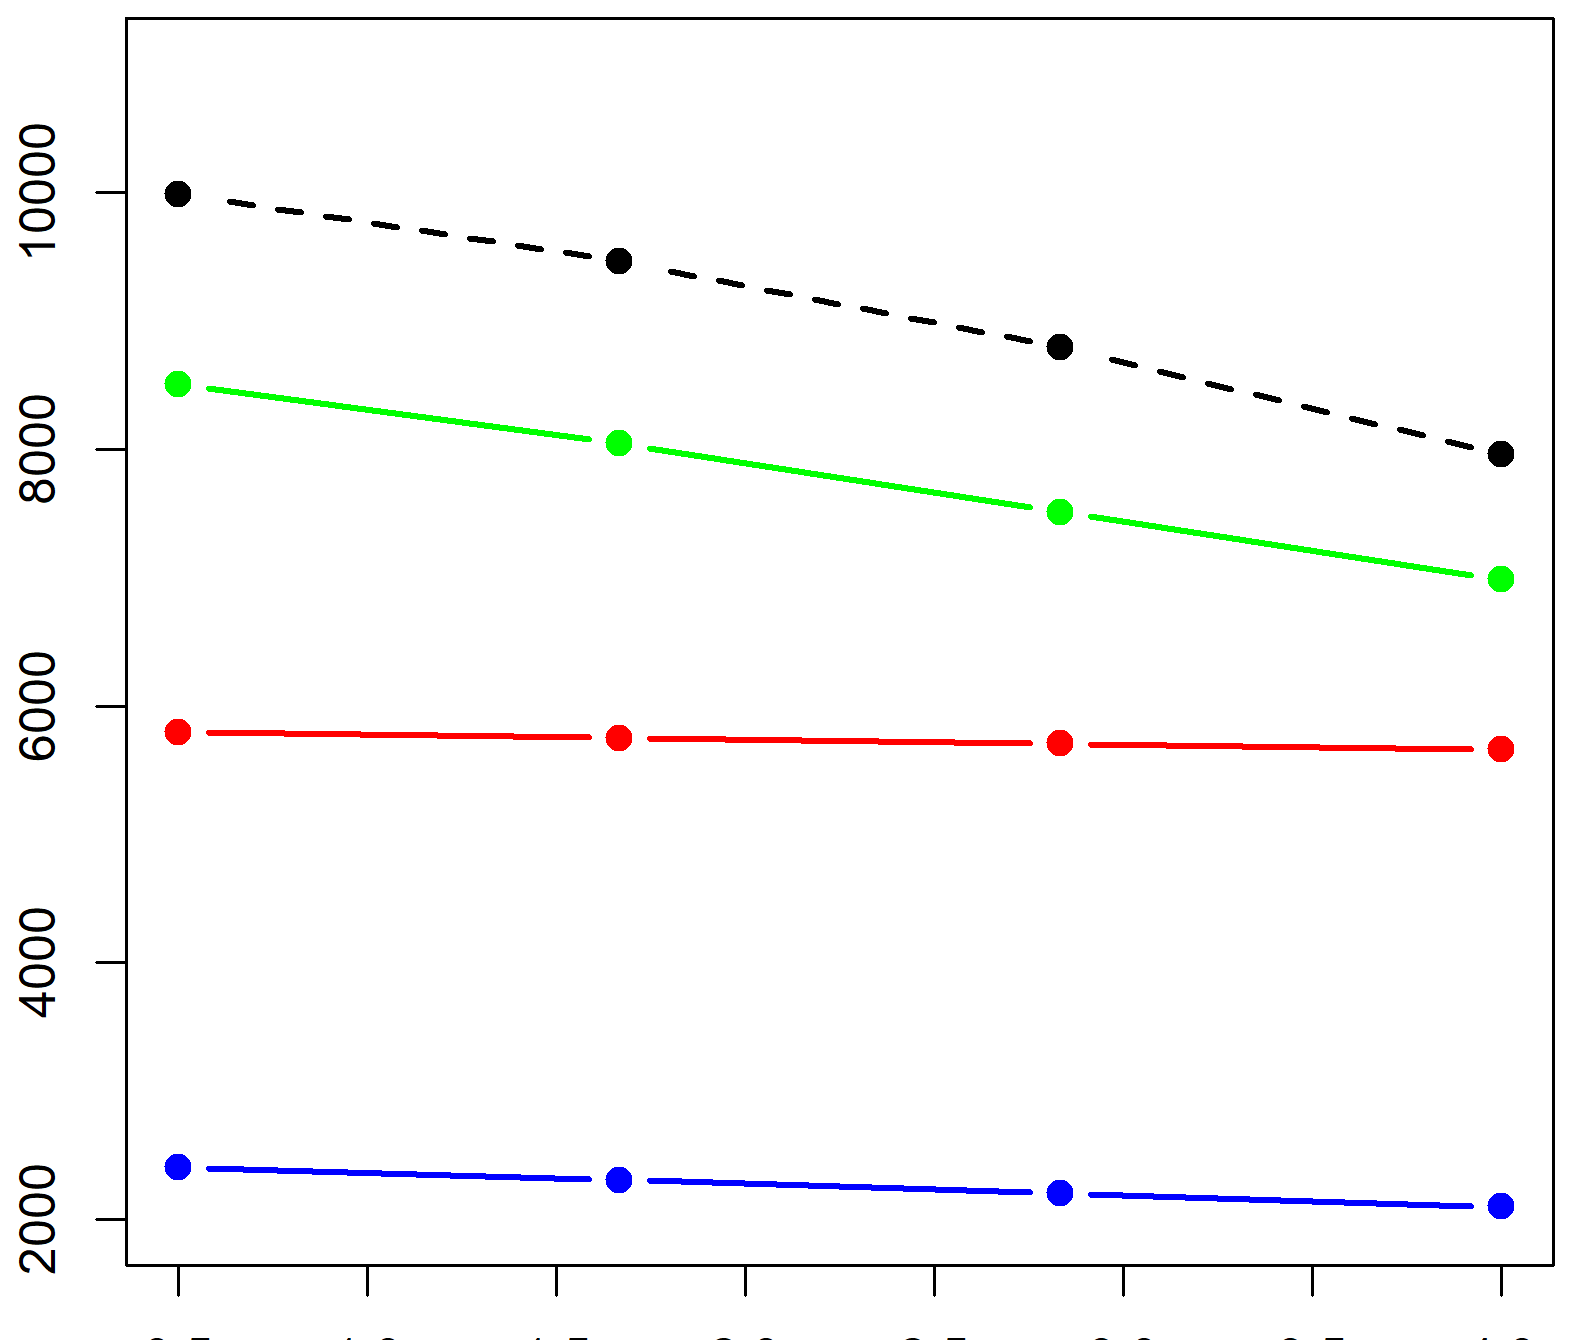
\includegraphics[scale=.6]{figures/example_figure.png}
    \caption{Example figure.}
    \label{fig:1}
\end{figure}
\section{Smoothing fan speed changes}

%%\section{design}

\lipsum[2-1]

\begin{lstlisting}[language=Java]
      for each webpage page in list of webpages {
          for each word p on page {
              ...
          }
      }
\end{lstlisting}
\section{Predicting future temperatures}

%%\section{Implementation}

\lipsum[2-1]
\section{Implementation details}
\subsection{Sensors, actuators}
\subsection{Optimisation}

%%\section{Evaluation}

\lipsum[2-1]
\section{Evaluation}

%%\section{Related}

\lipsum[2-1]

%%\section{Conclusion}

\lipsum[2-1]
\section{Conclusion}



%
%   References
%

\medskip

\bibliography{references.bib} 

\newpage

% %%%%%%%%%%%%%%%%%%%%%%%%%%%%%%%%%%%%%%%%%%%%%%%%%%%%%%%%%%
% %%%%%%%%%%%%%%%%%%%%%%%%%%%%%%%%%%%%%%%%%%%%%%%%%%%%%%%%%%
% TABLES
% %%%%%%%%%%%%%%%%%%%%%%%%%%%%%%%%%%%%%%%%%%%%%%%%%%%%%%%%%%
% %%%%%%%%%%%%%%%%%%%%%%%%%%%%%%%%%%%%%%%%%%%%%%%%%%%%%%%%%%

\end{document}